\section[BCS-theory]{The Bardeen-Cooper-Scheiffer theory of superconductivity}

This is essentially the many-particle version of the Cooper-problem.
Superconductivity: \todo{Sett inn figur}

Note that a non analytic function like this usually suggests that there is some phase-transition in the system, so we are essentially looking at a phase transition of the electron gas.
$T_C:$ A sharply defined temperature
\begin{equation}
\rho(T) =
\left\{
\begin{array}{ll}
	0  & \mbox{if } T<T_C \\
	\text{nonzero} & \mbox{if } T>T_C
\end{array}
\right.
\end{equation}


$T_C$ is denoted the critical temperature. Superconductivity was discovered experimentally in 1911 by Heike Kammerlingh Onnes in Leiden, measuring low-$T$ $\rho(T)$ in ultra pure Mercury (Hg). This was 15 years before the discovery of quantum mechanics. It turns out that the phenomena is purely a quantum effect. So in 1911, there was no hope of giving a correct explanation for what is happening. It took 46 years to figure out what is going on. The most important reasons for this, is that apart from having to invent quantum mechanics first, completely novel and radical ideas had to be formulated in order to solve the problem\footnote{From in the lecture: illustration of the Meissner effect. The Higgs providing a mass to the em-field in the metal blob drawn is the expectation value of the Cooper pair operator. Superconductivity is that the photon acquires a mass through the Higgs field, which is a cooper pair. Lots of analogs to the standard model.}. Historically, one important clue to figuring out what is happening, was the experimental observations that $T_C$ varied with ion mass. (Isotope substitution on elemental superconductors). This indicated that lattice-vibrations somehow were involved in the early discovered superconductors. (Recall that electron-phonon-coupling $\sim\frac{1}{\sqrt{M}}$). This ``isotope-effect'' was announced in 1950 on elemental Mercury, and the measured shift in $T_C$ was $0.01\mathrm{K}$, something that required very careful and precise measurements. We may guess what will happen with $T_C$ by appealing to what we found in the Cooper-problem, where we surmised a Cooper-pair dissociation temperature $T^* \sim  \Delta$ and 
\begin{equation}
\Delta = 2\hbar\omega_0\e^{-\frac1\lambda}
\end{equation}
$\omega_0$: A typical phonon-frequency, if we assume that the effective attractions originates with e-ph coupling. $\omega_0\sim \frac{1}{\sqrt{M}}$ $\rightarrow T^* \sim \frac{1}{\sqrt{M}}$.
This means that $\sqrt{M}T_C =$constant! This relation is validated very well in experiments on elemental superconductors such as Hg, Sn, and Tl. 
Previously, we have derived an effective e-e interaction, including Coulomb-interactions and e-ph--e interactions, $\tilde{V}_{\text{eff}}$.
\begin{align}
\begin{split}
\Ha &= \sum_{k, \sigma}\left(\ep_{k}-\mu\right)\cd_{ k\sigma}c_{k\sigma} \\ &+ \sum_{\stackrel{k,k',q}{\sigma, \sigma'}}\tilde{V}_{\text{eff}}\cd_{k+q, \sigma}\cd_{k'-q, \sigma'}c_{k', \sigma'}c_{k, \sigma}
\end{split}
\end{align}
Notice the global $\mathrm{U}(1)$-symmetry of this Hamiltonian.
This is on the standard form for a second-quantized electron-gas, now including the (potentially singular) effects of e-ph- coupling
\begin{equation}
\tilde{V}_{\text{eff}} = \frac{2|g_q|^2\omega_q}{\omega^2 - \omega_q^2} + V_\text{Coulomb}(q)
\end{equation}
\todo{Sett inn figure}

$\omega:$ Energy-transfer in scattering. $\omega = \ep_{k+q} - \ep_k, \quad \ep_{k'} = \ep_{k'-q} + \omega$.
The effect of the repulsive interaction can be calculated pertubatively. In any case, this repulsion is not a singular perturbation. We therefore set it aside for the moment, and consider
\begin{equation}
	\tilde{V}_{\text{eff}} = \frac{2|g_q|^2\omega_q}{\omega^2 - \omega_q^2}.
\end{equation}
This interaction as attractive ($<0$) if \[(\ep_{k+q}-\ep_k) ^2<\omega_q^2\] or \[(\ep_{k'-q}-\ep_{k'})^2 <\omega_q^2\]
We now focus on those scattering processes that give attraction between electrons. The processes giving repulsion do nothing more than what the Coulomb interaction does. We will include these effects later on. We now simplify this in a series of steps.
The scattering caused by the weak e-ph-e coupling can only take place in a thin shell around the Fermi-surface. Thus $\ep_{k}, \ep_{k'}, \ep_{k+q}, \ep_{k'-q}$ must all lie within a thin shell around the Fermi surface. Let us take a look at the relevant kinematics seen in \cref{fig:FS_shell}.
\begin{figure}
	\centering
	\begin{tikzpicture}[scale = 1.8]
	
	\coordinate (a) at (2, 2);
	\coordinate (k) at (1.8, 1.1);
	\coordinate (q) at (-1.6, 1);
	\coordinate (kprime) at (1.8, -1.1);
	
	\draw[dashed, blue] (a) circle (1.7);
	\draw[thick] (a) circle (2.);
	\draw[dashed, red] (a) circle (2.3);
	\draw[fill] (a) circle (0.03);
	
	\draw[thick, ->] (a) -- node[above]{\large $\vb k$} ++(k);
	\draw[thick, ->] (a)++(k) -- ++(q) node[above]{\large $\vb q$};
	\draw[thick, ->] (a) -- node[above]{\large$\vb k'$} ++(kprime);
	
	\draw[thick, ->] (a)++(kprime) -- ++($(0,0) -(q)$) node[above]{\large $-\vb q$};
	
	\node[anchor=east] at (3.7, 2) {\color{blue} \Large $\ep_F-\omega_0$};	
	
	\node[anchor=west] at (4.3, 2) {\color{red} \Large $\ep_F+\omega_0$};
\end{tikzpicture}
	\caption{Thin shell around the Fermi surface.}
	\label{fig:FS_shell}
\end{figure}
We see that in general, the state with momenta $k' -q$ will lie outside the shell, even if $\ep_{k}, \ep_{k'}, \ep_{k+q}$ lie \underline{within} the shell. There is an important special case where $\ep_{k'-q}$ will always lie within shell if $\ep_{k}, \ep_{k'}, \ep_{k+q}, \ep_{k'-q}$ is within shell, namely the case when $k' = -k$. 
This choice will this maximize the scattering phase-space for attractive interactions. We will retain only such terms: $k' = -k$. 

A \underline{second simplification}: $\sigma' = -\sigma$. The spatial extent of attractive interaction is small. We may essentially think of it (in real space) as an attractive Hubbard-interaction. Thus, we end up with the following simplified Hamiltonian
\begin{equation}
\label{eq:hamiltonian_attractive_hubbard_1}
\Ha = \sum_{k,\sigma}(\ep_k - \mu)\cd_{k\sigma}c_{k\sigma} + \sum_{k,q,\sigma}\tilde{V}_{\text{eff}}\cd_{k+q, \sigma}\cd_{-(k+q), -\sigma}c_{-k, -\sigma}c_{k\sigma}.
\end{equation}
Now redefine variables $k\rightarrow k', \quad k+q\rightarrow k, \quad \tilde{V}_{\text{eff}}\rightarrow V_{k,k'}/2$ (spin independent interaction). Thus we can write \cref{eq:hamiltonian_attractive_hubbard_1} as
\begin{equation}
\label{eq:Hamiltonian_BCS}
	\Ha = \sum_{k,\sigma}(\ep_k - \mu)\cd_{k\sigma}c_{k\sigma} + \sum_{k,k'}V_{k,k'}\cd_{k,\uparrow}\cd_{-k, \downarrow}c_{-k',\downarrow}c_{k,\uparrow},
\end{equation}
with $V_{k,k'}$ being attractive if $k,k'$ lie in a small vicinity of the Fermi-surface, and zero otherwise. 
\cref{eq:Hamiltonian_BCS} is the so called BCS-model of superconductivity. Althought it has been motivated by an attractive \underline{e-ph-e interaction}, the above model is in fact more general than that, and can be applied to any system with an effective (somehow) attractive electron-electron interaction.
This model in spirit is very much like the model we looked at for the Cooper-problem. The difference is that $V_{k,k'}$ in the BCS-model works between all electrons in a thin shell around the Fermi-surface, while the Cooper-problem only considered interactions between two such electrons.
The Hamiltonian can not be treated exactly. Moreover, from the Cooper-problem, there is every reason to believe that in order to get correct eigenvalues, we cannot use perturbations theory. We must therefore treat $\Ha$ both approximately and non-perturbatively. This is what we will do next.
We will transform this many-body problem to a self-consistent one-particle problem. This is done very much like what we do when we perform a mean-field approximation on spin-systems:
\begin{align}
\label{eq:mft_bcs}
\begin{split}
	c_{-k\downarrow}c_{k\uparrow} &= \underbrace{\ev{	c_{-k\downarrow}c_{k\uparrow}}}_{\equiv b_k} + \underbrace{c_{-k\downarrow}c_{k\uparrow} - \ev{	c_{-k\downarrow}c_{k\uparrow}}}_{\delta b_k} \\
	&= b_k + \delta b_k.
\end{split}
\end{align}
Here, $b_k$ is a statistical average \footnote{with respect to the ``correct'' Hamiltonian.}. Note that giving the $b$'s a finite expectation value breaks the \$\textbackslash\{\}mathrm\{U\}(1)\$-symmetry of the system. There is no way to gradually break this symmetry, it either happens or not. Note also that these expectations values are \underline{not} on the usual $\ev{c^\dagger c}$-form, and the question now is to answer whether such expectation values can exist or not.
Now insert the definitions in \cref{eq:mft_bcs} and the Hermitian conjugate into \cref{eq:Hamiltonian_BCS} and ignore terms $\mathcal{O}((\delta b)^2)$
Consider the interaction term:
\begin{align*}
\sum_{k,k'}V_{k,k'} \cd_{k,\uparrow}\cd_{-k, \downarrow}c_{-k',\downarrow}c_{k,\uparrow}
 &= \sum_{k,k'}V_{k,k'} \left(b_k^\dagger + \delta b_k^\dagger\right)\left(b_{k'} + \delta b_{k'}\vphantom{b_k^\dagger}\right)\\
&= \sum_{k,k'}V_{k,k'}\left(b_k^\dagger b_{k'} + b_k^\dagger\delta b_{k'} + \delta b_k^\dagger b_{k'}\right) + \mathcal{O}((\delta b)^2)\\
&\simeq \sum_{k,k'}V_{k,k'}\left(b_k^\dagger b_{k'} + b_k^\dagger c_{-k'\downarrow}c_{k'\uparrow} + b_{k'}\cd_{k\uparrow}\cd_{-k\downarrow} - 2b^\dagger_kb_{k'}\right).
\end{align*}

Next, definge
\begin{subequations}
	\label{eq:defs_delta}
\begin{align}
	\Delta_k\equiv&-\sum_{k'}V_{kk'}b_{k'} \label{eq:def_delta1} \\
	\Delta_k^\dagger\equiv&-\sum_{k}V_{kk'}b_k^\dagger. \label{eq:def_delta2}
\end{align}
\end{subequations}
Inserting these in definitions into the Hamiltonian gives
\begin{align}
\label{eq:BCS_MFT}
	\begin{split}
	\Ha = \sum_{k,\sigma}(\ep_k - \mu)\cd_{k\sigma}c_{k\sigma} 
	&-\sum_k\left[\Delta_k c_{k\uparrow}^\dagger c_{-k\downarrow}^\dagger + \Delta_k^\dagger c_{-k\downarrow c_{k\uparrow}}\right] \\
	&+ \sum_k \Delta_k b_k^\dagger.
	\end{split}
\end{align}

This is the mean-field approximation to the BCS-model, where $b_k$ (and hence $\Delta_k$) must be determined self-consistently, by minimizing the free energy of the system. We return to that below, but first we must diagonalize the Hamiltonian in \cref{eq:BCS_MFT}. Note that we now have terms like $c^\dagger c, \quad c^\dagger c^\dagger, $ and $cc$ in $\Ha$, reminiscent of what we had with boson-operators for the case of quantum antiferromagnets. We will now proceed along a similar route, but with the important difference that we are now considering fermions. Introduce new fermion-operators 
\begin{subequations}
	\label{eq:fermion_bogoliubov}
\begin{align}
\label{eq:def_eta} \eta_k &= u_k c_{k\uparrow} + v_k c_{-k\downarrow}^\dagger \\
\label{eq:def_gamma} \gamma_k &=u_kc_{-k\downarrow} - v_k c_{k\uparrow}
\end{align}
\end{subequations}
These operators are fermionic quasi-particles as linear combinations of spin-up and spin-down particles. Thus spin is not a correct quantum number for the new fermions. 
Note the minus sign in \cref{eq:def_gamma}. This transformations is required to preserve fermionic commutation relations, for instance 
\begin{equation}
\label{eq:acomm_eta}
	\acomm{\eta_k}{\eta_{k'}^\dagger} = \delta_{kk'},
\end{equation} $\eta_k, \gamma_k$ anticommute, \[\acomm{\eta_k}{\gamma_{k'}^\dagger} = 0\]. \[u_ku_{k'}\delta_{kk'} + v_kv_{k'}\delta_{kk'} =\delta_{kk'},\]
with the $+$-sign originating in anti-commutation relations. Thus\underline{$u_k^2 + v_k^2 = 1$}. We reach the same conclusion with $\acomm{\gamma_k}{\gamma_{k'}}=\delta_{kk'}$. This relation is the reason for the minus sign in front of $v_k$ in \cref{eq:def_gamma}!

\begin{equation}
\begin{pmatrix}
\eta_k \\ \gamma_k
\end{pmatrix}
 = 
 \overbrace{\begin{pmatrix}
 u_k & v_k \\ -v_k & u_k
 \end{pmatrix}}^{\equiv M}
 \begin{pmatrix}
c_{k\uparrow} \\ c_{-k\downarrow}^\dagger
 \end{pmatrix}
\end{equation}
With these signs, $\det M = u_k^2 + v_k^2 = 1$
\begin{align}
M =	\begin{pmatrix}
	u_k & v_k \\ -v_k & u_k
	\end{pmatrix}
	&&
M^T=	\begin{pmatrix}
	u_k & -v_k \\ v_k & u_k
	\end{pmatrix}
	&&
M^{-1}=	\begin{pmatrix}
	u_k & -v_k \\ v_k & u_k
	\end{pmatrix}
\end{align}

Thus, $M$ is a unitary transformation with the constraint $u_k^2 + v_k^2 = 1 \implies |u_k|, |v_k| \le 1$. This is very different from the ``squeezing'' transformation we used in the quantum AFM-case.
Going back to \cref{eq:fermion_bogoliubov}, we have
\begin{subequations}
\label{eq:matrix_rep}
\begin{align}
	\begin{pmatrix}
	\eta_k \\ \gamma_k
	\end{pmatrix}
	&= 
	\begin{pmatrix}
		u_k & v_k \\ -v_k & u_k
		\end{pmatrix}
	\begin{pmatrix}
	c_{k\uparrow} \\ c_{-k\downarrow}^\dagger
	\end{pmatrix} \\[1.5ex]
	\begin{pmatrix}
	\eta_k^\dagger \\ \gamma_k^\dagger
	\end{pmatrix}
	&= 
	\begin{pmatrix}
		u_k & v_k \\ -v_k & u_k
		\end{pmatrix}
	\begin{pmatrix}
	c_{k\uparrow}^\dagger \\ c_{-k\downarrow}
	\end{pmatrix} \\[1.5ex]
	\begin{pmatrix}
	c_{k\uparrow} \\ c_{-k\downarrow}^\dagger
	\end{pmatrix}
	&= 
	\begin{pmatrix}
		u_k & -v_k \\ v_k & u_k
		\end{pmatrix}
	\begin{pmatrix}
	\eta_k \\ \gamma_k
	\end{pmatrix} \\[1.5ex]
	\begin{pmatrix}
	c_{k\uparrow}^\dagger \\ c_{-k\downarrow}
	\end{pmatrix}
	&= 
	\begin{pmatrix}
		u_k & -v_k \\ v_k & u_k
		\end{pmatrix}
	\begin{pmatrix}
	\eta_k^\dagger \\ \gamma_k^\dagger
	\end{pmatrix} 
\end{align}
\end{subequations}

Insert this into the Hamiltonian \cref{eq:BCS_MFT},
\begin{align}
	\begin{split}
	\Ha &= \sum_k\left\{\left(\vphantom{\eta_k^\dagger}\ep_k-\mu\right)\left(u_k\eta_k^\dagger-v_k\gamma_k^\dagger\right)\left(\vphantom{\eta_k^\dagger}u_k\eta_k-v_k\gamma_k\right)\right. \\ 
	&+\left(\vphantom{\eta_k^\dagger}\ep_k-\mu\right)\left(\vphantom{\eta_k^\dagger}v_k\eta_k + u_k\gamma_k\right)\left(v_k\gamma_k^\dagger + u_k\gamma_k^\dagger\right) \\
	&-\Delta_k\left(u_k\eta_k^\dagger -v_k\gamma_k^\dagger\right)\left(\vphantom{\eta_k^\dagger}v_k\eta_k + u_k\gamma_k \right)\\
	&-\left. \Delta_k^\dagger\left(u_k\eta_k^\dagger + u_k\gamma_k^\dagger\right)\left(\vphantom{\eta_k^\dagger}u_k\eta_k-v_k\gamma_k\right) +\Delta_k b_k^\dagger \vphantom{\left(\eta_k^\dagger\right.} \right\}
	\end{split}
\end{align}
As in the quantum antiferromagnet-case, we now collect terms of different types:
\begin{subequations}
\begin{align}
	\eta_k^\dagger\eta_k :& \left(\ep_k-\mu\right)u_k^2 - u_kv_k\left(\Delta_k+\Delta_k^\dagger\right)\label{eq:term_1} \\
	\gamma_k^\dagger\gamma_k :& \left(\ep_k - \mu\right)v_k^2 + +u_kv_k\left(\Delta_k + \Delta_k^\dagger\right) \label{eq:term_2}\\
	\eta_k\eta_k^\dagger :&  \left(\ep_k-\mu\right)v_k^2 \\
	\gamma_k\gamma_k^\dagger:& \left(\ep_k-\mu\right)u_k^2 \\
	\gamma_k^\dagger\eta_k :&-2\left(\ep_k-\mu\right)u_kv_k + \Delta_k v_k^2- \Delta_k^\dagger u_k^2\label{eq:term_3} \\
	\label{eq:term_4}
	\eta_k^\dagger\gamma_k :& -2\left(\ep_k-\mu\right)u_kv_k - \Delta_k u_k^2 + v_k^2\Delta_k^\dagger 
\end{align}
\end{subequations}
Using the anticommutation relations in \cref{eq:acomm_eta}, and the corresponding for $\gamma_k$, we may express \cref{eq:term_1,eq:term_2} as
\begin{subequations}
	\begin{align}
		\eta_k^\dagger\eta_k :& \left(\ep_k-\mu\right)\left(u_k^2-v_k^2\right)-u_kv_k\left(\Delta_k+\Delta_k^\dagger\right) \\
		\gamma_k^\dagger\gamma_k :& \left(\ep_k - \mu\right)\left(v_k^2-u_k^2\right)  +u_kv_k\left(\Delta_k + \Delta_k^\dagger\right) 
	\end{align}
\end{subequations}
These are the same, except opposite sign. Adjust $u_k, v_k$ such that the coefficients in front of \cref{eq:term_3, eq:term_4} are zero. Fortunately, these two equations are just complex conjugate of each other, so if one is fulfilled, so is the other.
If we set these two to $0$, we have
\begin{align}
		-2\left(\ep_k - \mu\right)u_kv_k &= u_k^2\Delta_k - v_k^2\Delta_k^\dagger \\
		-2\left(\ep_k - \mu\right)u_kv_k &= u_k^2\Delta_k^\dagger-v_k^2\Delta_k^\dagger.
\end{align}
By adding these two equations, we get
\begin{align*}
-4\underbrace{\left(\ep_k-\mu\right)}_{\equiv\tilde{\ep}_k}u_kv_k &= \left(u_k^2-v_k^2\right)\left(\Delta_k+\Delta_k^\dagger\right) \\
\Delta_k+\Delta_k^\dagger &=  2\Re{\Delta_k} \equiv 2\td_k \\
-2\te_ku_kv_k &= \left(u_k^2-v_k^2\right)\td_k
\end{align*}
Since we have $u_k^2+v_k^2 = 1$, we may write 
\begin{align*}
	u_k &= \cos\theta \\
	v_k &=\sin\theta \\
	-\te_k\sin2\theta &= \td_k\cos2\theta 
\end{align*}
\begin{equation}
\label{eq:BCS_theta}
	\tan 2\theta =-\frac{\td_k}{\te_k}
\end{equation}
This is an equation for $\theta$, and thus $u_k, v_k$, which gives coefficients of $\gamma_k^\dagger\eta_k, \eta_k^\dagger\gamma_k$ equal to zero. 
Choose $\td_k \ge0$
\begin{align*}
	\tan2\theta <0 ;&\quad \te >0 \\
	\tan2\theta >0 ;&\quad \te <0 \\
	\frac{\sin[2](2\theta)}{\cos[2](2\theta)} &= \left(\frac{\td_k}{\te_k}\right)^2 \equiv b^2 \\
	\cos[2](2\theta) &= \frac{1}{1+b^2} \\
	\cos(2\theta) &= \left\{\begin{array}{ll} \frac{-1}{\sqrt{1+b^2}}\, ; \quad \te >0 \\ \frac{1}{\sqrt{1+b^2}}\, ; \quad \te <0
	\end{array}\right.
\end{align*}
Coefficient in front of $\eta_k^\dagger\eta_k$:
\begin{align*}
\te_k\cos2\theta - \td_k\sin2\theta &= \cos(2\theta)\left(\te_k+\left(\frac{\td_k}{\te_k}\right)^2\right) \\
&= -\frac{\sign\te_k}{\te_k}\frac{\left(\te_k^2 + \td_k^2\right)}{(1+b^2)^{\frac12}} \\
&= -\frac{\sign\te_k}{\frac{\te_k}{|\te_k|}}\left(\te_k^2 + \td_k^2\right)^\frac12 \\
&= -\left(\te_k^2 + \td_k^2\right)^\frac12
\end{align*}
Coefficient in front of $\gamma_k^\dagger\gamma_k$: $\left(\te_k^2 + \td_k^2\right)^\frac12$. Thus, we have finally diagonalized the Hamiltonian 
\begin{equation}
\Ha = \sum_k\left[2\left(\ep_k-\mu\right) + \Delta_kb_k^\dagger + E_k\left(\gamma_k^\dagger\gamma_k - \eta_k^\dagger\eta_k\right)\right],
\end{equation}
where the summation over spins has been made, and with
\begin{equation}
E_k\equiv \left(\te_k^2 + \td_k^2\right)^\frac12.
\end{equation}
$b_k$ and $\td_k$ are as yet undetermined. They will have to be determined by minimizing the free energy of this system. 
The long-lived fermionic excitation are described by $(\eta_k, \eta_k^\dagger),\,(\gamma_k, \gamma_k^\dagger)$.
\todo{Sjekk at fortegnene er riktige på eta/gamma}
\begin{align}
\Ha &= E_0 + \sum_k E_k\left(\gamma_k^\dagger\gamma_k - \eta_k^\dagger\eta_k \right) \\
E_0 &= \sum_k \left[2\left(\ep_k-\mu\right) + \Delta_kb_k^\dagger\right]
\end{align}
If we have a fermionic system with a Hamiltonian \[\Ha = \sum_k(\ep_k-\mu)c^\dagger_kc_k,\] the grand canonical partition function is given by
\begin{equation}
\Z_g = \prod_k\left(1+\e^{-\beta(\ep_k-\mu)}\right).
\end{equation}
Is the present case, this gives 
\begin{equation}
\Z_g =\e^{-\beta E_0}\prod_k\left(1+\e^{\beta E_k}\right)\left(1+\e^{-\beta E_k}\right).
\end{equation}
In the limit of large number of particles, all ensembles are equivalent. To expedite th computations, we will consider $\Z_g$ ti be equal to $\Z = \e^{-\beta F}$, where $F$ is the Helmholz free energy for a system.
\begin{equation}
\label{eq:BCS_free_energy}
F = E_0 -\frac1\beta\sum_k\left[\ln(1+\e^{-\beta E_k}) + \ln(1+\e^{\beta E_k})\right]
\end{equation}

We now minimize with respect to $\Delta_k$ or $b_k^\dagger$ for a particular value of $k$. It does not matter which one of these we use. We look for 
\begin{equation}
\pdv{F}{\Delta_k} = 0,
\end{equation}
or
\begin{equation*}
b_k^\dagger - \frac1\beta\left(\frac{1}{1+\e^{-\beta E_k}}(-\beta)\pdv{E_k}{\Delta_k}\e^{-\beta E_k} + \frac{1}{1+\e^{\beta E_k}}(\beta)\pdv{E_k}{\Delta_k}\e^{\beta E_k}\right) = 0
\end{equation*}
\begin{align*}
b_k^\dagger &= \pdv{E_k}{\Delta_k}\left(\frac{\e^x}{1+e^x} -\frac{\e^{-x}}{1+e^{-x}}\right) \\
&= \pdv{E_k}{\Delta_k}\cdot\tanh(\frac{x}{2})\, ;\quad x= \beta E_k \\
\pdv{E_k}{\Delta_k} &= \frac{\Delta_k}{\sqrt{\te_k^2 + \Delta_k^2}},
\end{align*}
where we have set $\Delta_k$ to be real, such that $\td_k = \Delta_k$.
\begin{equation}
b_k^\dagger = \frac{\Delta_k}{\sqrt{\te_k^2 + \Delta_k^2}}\tanh(\frac{\beta E_k}{2})
\end{equation}
We close this to an equation for $\Delta_k$ by using the definitions in \cref{eq:defs_delta} to obtain
\begin{tcolorbox}
	\begin{align}
	\label{eq:BCS_gap}
	\Delta_k &= -\sum_{k'}V_{kk'}\Delta_{k'}\chi_{k'} \\
	\chi_k &= \frac{1}{\left(\te_k^2+\Delta_k^2\right)^\frac12}\tanh(\frac{\beta E_k}{2})
	\end{align}
\end{tcolorbox}
This is the so-called BCS gap-equation. The reason for this name that it is an equation for $\Delta_k$, which represents a gap in the excitation-spectrum. To see this, we first consider the excitation spectrum at $\Delta_k = 0$, depicted in \cref{fig:excitation_spectrum_no_delta}
\begin{figure}
	\centering
	\begin{subfigure}{0.49\linewidth}
		\centering
		\begin{tikzpicture}[scale=0.65]

\begin{axis}[
ticks = none,
legend style={font =\Large,at={(1,0.7)}},
%ytick = {1},
%yticklabels = {$\varepsilon_f$},
%xtick = {0},
%xticklabels ={,,},
xlabel = \Large $k$,
axis lines = left,
x label style={at={(axis description cs:1,0.5)}, anchor = west},
ymin = -1.5,
ymax= 2,
xmax = 2.5,
axis x line shift = -1.5
%y label style={at={(axis description cs:0.15,1)},rotate=-90,anchor=south},
%xlabel = $x$,
%sylabel = {$f(x)$},
]
%%Below the red parabola is defined
%\addplot [
%thick,
%domain=0:1.4, 
%samples=100, 
%color=red,
%]{1/2 * (1 + x^2 + sqrt((x^2 - 1)^2 + 0.1))};

\coordinate (b) at (axis cs:1,0) ;
\node[circle, fill, inner sep =1.8pt] at (b){};
\node[anchor = north] at (axis cs:1.05,-0.1){\Large $k_F$};

\addplot [
thick,
domain=0:3, 
samples=100, 
color=green!50!black,
]{x^2-1};

%%Here the blue parabloa is defined
%\addplot [
%thick,
%domain=0:1.4, 
%samples=100, 
%color=blue,
%]{1/2 * (1 + x^2 - sqrt((x^2 - 1)^2 + 0.1))};

%
%\addplot[
%thick,
%domain = 0:1.4,
%samples = 100,
%dashed
%]{1};

\addlegendentry{${\te_k}$}
%\addlegendentry{$\mathbf{\varepsilon_k}$}
%\addlegendentry{$\mathbf{E_k^-}$}
\end{axis}
\end{tikzpicture}
		\subcaption{$\te_k$}
	\end{subfigure}
	\begin{subfigure}{0.49\linewidth}
		\centering
		\begin{tikzpicture}[scale = 0.65]

\begin{axis}[
ticks = none,
legend style={font =\Large,at={(1,0.7)}},
%ytick = {1},
%yticklabels = {$\varepsilon_f$},
%xtick = {0},
%xticklabels ={,,},
xlabel = \Large $k$,
axis lines = left,
x label style={at={(axis description cs:1,0.5)}, anchor = west},
ymin = -1.5,
ymax= 2,
xmax = 2.5,
axis x line shift = -1.5
%y label style={at={(axis description cs:0.15,1)},rotate=-90,anchor=south},
%xlabel = $x$,
%sylabel = {$f(x)$},
]
%%Below the red parabola is defined
%\addplot [
%thick,
%domain=0:1.4, 
%samples=100, 
%color=red,
%]{1/2 * (1 + x^2 + sqrt((x^2 - 1)^2 + 0.1))};

\coordinate (b) at (axis cs:1,0) ;
\node[circle, fill, inner sep =1.8pt] at (b){};
\node[anchor = north] at (axis cs:1.05,-0.1){\Large $k_F$};


\addplot [
thick,
domain=0:3, 
samples=100, 
color=red!50!black,
]{abs(x^2-1)};

%%Here the blue parabloa is defined
%\addplot [
%thick,
%domain=0:1.4, 
%samples=100, 
%color=blue,
%]{1/2 * (1 + x^2 - sqrt((x^2 - 1)^2 + 0.1))};

%
%\addplot[
%thick,
%domain = 0:1.4,
%samples = 100,
%dashed
%]{1};

\addlegendentry{${|\te_k|}$}
%\addlegendentry{$\mathbf{\varepsilon_k}$}
%\addlegendentry{$\mathbf{E_k^-}$}
\end{axis}
\end{tikzpicture}
		\subcaption{$|\te_k|$}
	\end{subfigure}

	\caption{Excitation spectrum at $\Delta_k = 0$}
	\label{fig:excitation_spectrum_no_delta}
\end{figure}
Note that on the Fermi-surface ($k = k_F$), there is zero gap in the excitation spectrum $\Delta_k =0$. 
\begin{figure}
	\centering
	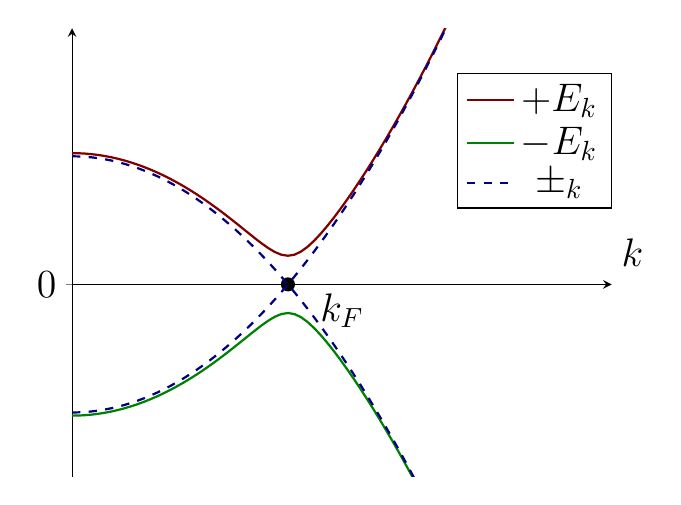
\begin{tikzpicture}

\begin{axis}[
%ticks = none,
legend style={font =\Large,at={(1,0.9)}},
ytick = {0},
yticklabels = {\Large $0$},
xtick = {0},
xticklabels ={,,},
xlabel = \Large $k$,
axis lines = left,
x label style={at={(axis description cs:1,0.5)}, anchor = west},
ymin = -1.5,
ymax= 2,
xmax = 2.5,
axis x line shift = -1.5
%y label style={at={(axis description cs:0.15,1)},rotate=-90,anchor=south},
%xlabel = $x$,
%sylabel = {$f(x)$},
]
%%Below the red parabola is defined
%\addplot [
%thick,
%domain=0:1.4, 
%samples=100, 
%color=red,
%]{1/2 * (1 + x^2 + sqrt((x^2 - 1)^2 + 0.1))};

\coordinate (b) at (axis cs:1,0) ;
\node[circle, fill, inner sep =1.8pt] at (b){};
\node[anchor = north] at (axis cs:1.25,-0.0){\Large $k_F$};


\addplot [
thick,
domain=0:3, 
samples=100, 
color=red!50!black,
]{sqrt((x^2-1)^2 + 0.05)};

\addplot [
thick,
domain=0:3, 
samples=100, 
color=green!50!black,
]{-sqrt((x^2-1)^2 + 0.05)};


\addplot [
thick,dashed,
domain=0:3, 
samples=100, 
color=blue!50!black,
]{(x^2-1)};
\addplot [
thick,dashed,
domain=0:3, 
samples=100, 
color=blue!50!black,
]{-(x^2-1)};


%%Here the blue parabloa is defined
%\addplot [
%thick,
%domain=0:1.4, 
%samples=100, 
%color=blue,
%]{1/2 * (1 + x^2 - sqrt((x^2 - 1)^2 + 0.1))};

%
%\addplot[
%thick,
%domain = 0:1.4,
%samples = 100,
%dashed
%]{1};

\addlegendentry{${+E_k}$}
\addlegendentry{$-E_k$}
\addlegendentry{$\pm \te_k$}
\end{axis}
\end{tikzpicture}
	\caption{$\Delta_k \ne 0$ represents a gap in the excitation spectrum at the Fermi surface, here greatly exaggerated. The difference in the minimum of $+E_k$ and the maximum of $-E_k$ is $2\Delta_k$. This gap always tracks the Fermi surface. }
	\label{fig:BCS_gap}
\end{figure}
From \cref{fig:BCS_gap}, we see that $\Delta_k$ represents a gap \underline{on the Fermi-surface} in the excitation spectrum of the Bogoliubov fermions.
We will now solve \cref{eq:BCS_gap} for the same model for $V_{kk'}$ that we used in the Cooper problem, namely a constant attractive potential in a thin shell around the Fermi-surface. With the understanding that $k,k'$ lie within this thin shell, we have 
\begin{equation}
	\Delta_k = V\sum_{k'}\Delta_{k'}\chi_{k'}
\end{equation}
This means that $\Delta_k$ is independent of $k$, and we can divide by $\Delta =\Delta_k$ and get
\begin{equation}
	1 = V\sum_{k'}\frac{1}{\left(\te_{k'}^2+\Delta^2\right)^\frac12}\tanh(\frac{\beta E_{k'}}{2}).
\end{equation}
Now use 
\begin{equation}
\sum_{k}g(\te_k) = \int_{-\infty}^\infty\dd\ep\sum_k\delta(\ep-\te_k)g(\te) = \int_{-\infty}^{\infty}\dd\ep N(\ep)g(\ep),
\end{equation}
\begin{equation}
	1 = V\int_{-\omega_0}^{\omega_0}\dd\ep \frac{N(\ep)}{\sqrt{\ep^2 + \Delta^2}}\tanh(\frac{\beta\sqrt{\ep^2+\Delta^2}}{2})
\end{equation}

